% TODO: Negations-Besipiel beim ZK (schrittweise def. einer induktiven ZK-Fkt.)

% Define a global usable date. Must come before StyleTut
\newcommand{\mydate}{25.11.2016}

% Comment/uncomment this line to toggle handout mode
\newcommand{\handout}{}


% Das ist der KIT-Stil
%\usepackage{../TutTexbib/beamerthemekit}
\usepackage[deutsch,titlepage0]{../TutTexbib/KIT/beamerthemeKITmod}
\TitleImage[width=\titleimagewd]{../figures/titlepage.jpg}
%\usetheme[deutsch,titlepage0]{KIT}

% Include PDFs
\usepackage{pdfpages}

% Libertine font (Original GBI font)
\usepackage{libertine}
%\renewcommand*\familydefault{\sfdefault}  %% Only if the base font of the document is to be sans serif

% Nicer math symbols
\usepackage{eulervm}
%\usepackage{mathpazo}
\renewcommand\ttdefault{cmtt} % Computer Modern typewriter font, see lecture slides.

%% Deutsche Silbentrennung und Beschriftungen
\usepackage[ngerman]{babel}



\usepackage{csquotes}



%% Anzeigetiefe für Inhaltsverzeichnis: 1 Stufe
\setcounter{tocdepth}{1}

%% Schönere Schriften
\usepackage[TS1,T1]{fontenc}

%% Bibliothek für Graphiken
\usepackage{graphicx}

%% der wird sowieso in jeder Datei gesetzt
%%\graphicspath{{../figures/}}

%% Hyperlinks
\usepackage{hyperref}
% I don't know why, but this works and only includes sections and NOT subsections in the pdf-bookmarks.
\hypersetup{bookmarksdepth=subsection} 

%\usepackage{lmodern}
\usepackage{colortbl}
\usepackage[absolute,overlay]{textpos}
\usepackage{listings}
\usepackage{forloop}
%\usepackage{algorithmic} % PseudoCode package 

\usepackage{tikz}
\usetikzlibrary{matrix}
\usetikzlibrary{arrows.meta}
\usetikzlibrary{automata}
\usetikzlibrary{tikzmark}

% Needed for gbi-macros
\usepackage{xspace}

%%%%%%%%%%%% INHALT %%%%%%%%%%%%%%%%

%% Wochennummer
\newcounter{weeknum}



%% Titelinformationen
\title[GBI-Tutorium \mytutnumber, Woche \theweeknum]{Grundbegriffe der Informatik \\ Tutorium \mytutnumber}

\subtitle{Woche \theweeknum \ | \mydate{\theweeknum} \\ \myname \ \  \normalfont (\mailto{\mymail})}
\author[\myname]{\myname}
\institute{KIT -- Karlsruher Institut für Technologie}
\date{\mydate{\theweeknum}\ }

% Modified, DJ (better safe than sorry)
\AuthorTitleSep{ – }

%% Titel einfügen
\newcommand{\titleframe}{\frame{\titlepage}}

%% Alles starten mit \starttut{X}
\newcommand{\starttut}[1]{\setcounter{weeknum}{#1}\titleframe\frame{\frametitle{Inhalt}\tableofcontents} \AtBeginSection[]{%
\begin{frame}
	\tableofcontents[currentsection]
\end{frame}\addtocounter{framenumber}{-1}}}


\newcommand{\framePrevEpisode}{
	\begin{headframe}
		\mylasttimestext
	\end{headframe}
}

%% Legacy: Lastframe. Not for further usage!
\newcommand{\lastframetitled}[5]{
	\frame[plain]{
		\vspace{-#2pt}
		\begin{figure}[H]
			\centering
			\LARGE \textbf{\textsc{#5}} \\
			\vspace{.2\baselineskip}
			\includegraphics[scale=#1]{#3}
			\vspace{-7pt}
			\caption{ \texttt{\url{#4}} }
		\end{figure} 
	}
}
\newcommand{\lastframe}[4]{\xkcdframe{#1}{#2}{#3}{#4}{}}
\newcommand{\xkcdframe}[5]{
	\frame[plain]{
		\vspace{-#2pt}
		\begin{figure}[H]
			\centering
			\includegraphics[scale=#1]{#3}
			\vspace{-7pt}
			\caption{ \texttt{\url{#4}} }
			\vspace{5pt}
			#5
		\end{figure} 
	}
}

%% Wörter
\newcommand{\code}[1]{$\mathbf{#1}$}

%% Sterne

\newcounter{starsc}
\newcommand{\stars}[1]{
	\hfill
	\begin{minipage}{100px}
		\forloop{starsc}{0}{\value{starsc} < #1}%
		{%
			
\includegraphics[scale=0.05]{star-full.pdf} \hspace*{1px}
		}%
		\forloop{starsc}{\value{starsc}}{\value{starsc} < 5}%
		{%
			
\includegraphics[scale=0.05]{star-empty.pdf} \hspace*{1px}
		}
		\vspace*{2px}
	\end{minipage}
}

% No stars for me...
\renewcommand{\stars}[1]{}

\newcommand{\slideThanks}{
	\begin{frame}
		\frametitle{Credits}
		\begin{block}{}
			Vorgänger dieses Foliensatzes wurden erstellt von:\\[1em]
			Thassilo Helmold \\
			Philipp Basler \\
			Nils Braun \\
			Dominik Doerner \\
			Ou Yue \\
		\end{block}
	\end{frame}
}

%% Verbatim
\usepackage{moreverb}
%% Beamer-Klasse im korrekten Modus
\ifdefined \handout
\documentclass[handout]{beamer} % Handout mode
\else
\documentclass{beamer}
\fi

%% UTF-8-Encoding
\usepackage[utf8]{inputenc}

% % \bigtimes abgeschrieben von http://tex.stackexchange.com/questions/14386/importing-a-single-symbol-from-a-different-font
% \DeclareFontFamily{U}{mathx}{\hyphenchar\font45}
% \DeclareFontShape{U}{mathx}{m}{n}{
%       <5> <6> <7> <8> <9> <10> gen * mathx
%       <10.95> mathx10 <12> <14.4> <17.28> <20.74> <24.88> mathx12
%       }{}
% \DeclareSymbolFont{mathx}{U}{mathx}{m}{n}
% \DeclareMathSymbol{\bigtimes}{\mathop}{mathx}{161}

\RequirePackage{xcolor}

\def\9{\square}
%\def\9{\blank}

% f"ur Aussagenlogik
\colorlet{alcolor}{blue}
\RequirePackage{tikz}
\usetikzlibrary{arrows.meta}
\newcommand{\alimpl}{\mathrel{\tikz[x={(0.1ex,0ex)},y={(0ex,0.1ex)},>={Classical TikZ Rightarrow[]}]{\draw[alcolor,->,line width=0.7pt,line cap=round] (0,0) -- (15,0);\path (0,-6);}}}
\newcommand{\aleqv}{\mathrel{\tikz[x={(0.1ex,0ex)},y={(0ex,0.1ex)},>={Classical TikZ Rightarrow[]}]{\draw[alcolor,<->,line width=0.7pt,line cap=round] (0,0) -- (18,0);\path (0,-6);}}}
\newcommand{\aland}{\mathbin{\raisebox{-0.6pt}{\rotatebox{90}{\texttt{\color{alcolor}\char62}}}}}
\newcommand{\alor}{\mathbin{\raisebox{-0.8pt}{\rotatebox{90}{\texttt{\color{alcolor}\char60}}}}}
%\newcommand{\ali}[1]{_{\mathtt{\color{alcolor}#1}}}
\newcommand{\alv}[1]{\mathtt{\color{alcolor}#1}}
\newcommand{\alnot}{\mathop{\tikz[x={(0.1ex,0ex)},y={(0ex,0.1ex)}]{\draw[alcolor,line width=0.7pt,line cap=round,line join=round] (0,0) -- (10,0) -- (10,-4);\path (0,-8) ;}}}
\newcommand{\alP}{\alv{P}} %ali{#1}}
%\newcommand{\alka}{\negthinspace\hbox{\texttt{\color{alcolor}(}}}
\newcommand{\alka}{\negthinspace\text{\texttt{\color{alcolor}(}}}
%\newcommand{\alkz}{\texttt{\color{alcolor})}}\negthinspace}
\newcommand{\alkz}{\text{\texttt{\color{alcolor})}}\negthinspace}
\newcommand{\AAL}{A_{AL}}
\newcommand{\LAL}{\hbox{\textit{For}}_{AL}}
\newcommand{\AxAL}{\hbox{\textit{Ax}}_{AL}}
\newcommand{\AxEq}{\hbox{\textit{Ax}}_{Eq}}
\newcommand{\AxPL}{\hbox{\textit{Ax}}_{PL}}
\newcommand{\AALV}{\hbox{\textit{Var}}_{AL}}
\newcommand{\MP}{\hbox{\textit{MP}}}
\newcommand{\GEN}{\hbox{\textit{GEN}}}
\newcommand{\W}{\ensuremath{\hbox{\textbf{w}}}\xspace}
\newcommand{\F}{\ensuremath{\hbox{\textbf{f}}}\xspace}
\newcommand{\WF}{\ensuremath{\{\W,\F\}}\xspace}
\newcommand{\val}{\hbox{\textit{val}}}
\newcommand{\valDIb}{\val_{D,I,\beta}}

\newcommand*{\from}{\colon}

% die nachfolgenden Sachen angepasst an cmtt
\newlength{\ttquantwd}
\setlength{\ttquantwd}{1ex}
\newlength{\ttquantht}
\setlength{\ttquantht}{6.75pt}
\def\plall{%
  \tikz[line width=0.67pt,line cap=round,line join=round,baseline=(B),alcolor] {
    \draw (-0.5\ttquantwd,\ttquantht) -- node[coordinate,pos=0.4] (lll){} (-0.25pt,-0.0pt) -- (0.25pt,-0.0pt) -- node[coordinate,pos=0.6] (rrr){} (0.5\ttquantwd,\ttquantht);
    \draw (lll) -- (rrr);
    \coordinate (B) at (0,-0.35pt);
  }%
}
\def\plexist{%
  \tikz[line width=0.67pt,line cap=round,line join=round,baseline=(B),alcolor] {
    \draw (-0.9\ttquantwd,\ttquantht) -- (0,\ttquantht) -- node[coordinate,pos=0.5] (mmm){} (0,0) --  (-0.9\ttquantwd,0);
    \draw (mmm) -- ++(-0.75\ttquantwd,0);
    \coordinate (B) at (0,-0.35pt);
  }\ensuremath{\,}%
}
\let\plexists=\plexist
\newcommand{\NT}[1]{\ensuremath{\langle\mathrm{#1} \rangle}}

\newcommand{\CPL}{\text{\itshape Const}_{PL}}
\newcommand{\FPL}{\text{\itshape Fun}_{PL}}
\newcommand{\RPL}{\text{\itshape Rel}_{PL}}
\newcommand{\VPL}{\text{\itshape Var}_{PL}}
\newcommand{\ATer}{A_{\text{\itshape Ter}}}
\newcommand{\ARel}{A_{\text{\itshape Rel}}}
\newcommand{\AFor}{A_{\text{\itshape For}}}
\newcommand{\LTer}{L_{\text{\itshape Ter}}}
\newcommand{\LRel}{L_{\text{\itshape Rel}}}
\newcommand{\LFor}{L_{\text{\itshape For}}}
\newcommand{\NTer}{N_{\text{\itshape Ter}}}
\newcommand{\NRel}{N_{\text{\itshape Rel}}}
\newcommand{\NFor}{N_{\text{\itshape For}}}
\newcommand{\PTer}{P_{\text{\itshape Ter}}}
\newcommand{\PRel}{P_{\text{\itshape Rel}}}
\newcommand{\PFor}{P_{\text{\itshape For}}}

\newcommand{\plka}{\alka}
\newcommand{\plkz}{\alkz}
%\newcommand{\plka}{\plfoo{(}}
%\newcommand{\plkz}{\plfoo{)}}
\newcommand{\plcomma}{\hbox{\texttt{\color{alcolor},}}}
\newcommand{\pleq}{{\color{alcolor}\,\dot=\,}}

% MODIFIED (DJ)
% previously: \newcommand{\plfoo}[1]{\mathtt{\color{alcolor}#1}}
\newcommand{\plfoo}[1]{\texttt{\color{alcolor}#1}}

\newcommand{\plc}{\plfoo{c}}
\newcommand{\pld}{\plfoo{d}}
\newcommand{\plf}{\plfoo{f}}
\newcommand{\plg}{\plfoo{g}}
\newcommand{\plh}{\plfoo{h}}
\newcommand{\plx}{\plfoo{x}}
\newcommand{\ply}{\plfoo{y}}
\newcommand{\plz}{\plfoo{z}}
\newcommand{\plR}{\plfoo{R}}
\newcommand{\plS}{\plfoo{S}}

\newcommand{\bv}{\mathrm{bv}}
\newcommand{\fv}{\mathrm{fv}}

%\newcommand{\AxAL}{\hbox{\textit{Ax}}_{AL}}
%\newcommand{\AALV}{\hbox{\textit{Var}}_{AL}}

%\renewcommand{\#}[1]{\literal{#1}}
\newcommand{\A}{\mathcal{A}}
\newcommand{\Adr}{\text{Adr}}
\newcommand{\ar}{\mathrm{ar}}
\newcommand{\ascii}[1]{\literal{\char#1}}
%\newcommand{\assert}[1]{\text{/\!\!/\ } #1}
\newcommand{\assert}[1]{\colorbox{black!7!white}{\ensuremath{\{\;#1\;\}}}}
\newcommand{\Assert}[1]{$\langle$\textit{#1}$\rangle$}
\newcommand{\B}{\mathcal{B}}
\newcommand{\bfmod}{\mathbin{\kw{ mod }}}
\newcommand{\bb}{{\text{bb}}}
\def\bottom{\hbox{\small$\pmb{\bot}$}}
\newcommand{\card}[1]{|#1|}
%\newcommand{\cod}{\mathop{\text{cod}}}  % ist in thwmathabbrevs
\newcommand{\Conf}{\mathcal{C}}
\newcommand{\define}[1]{\emph{#1}}
%\renewcommand{\dh}{d.\,h.\@\xspace}
%\newcommand{\Dh}{D.\,h.\@\xspace}
%\newcommand{\engl}[1]{engl.\xspace\emph{#1}}
\newcommand{\eps}{\varepsilon}
%\newcommand{\evtl}{evtl.\@\xspace}
\newcommand{\fbin}{\text{bin}}
\newcommand{\finv}{\text{inv}}
\newcommand{\fnum}{\text{num}}
\newcommand{\fNum}{{\text{Num}}}
\newcommand{\frepr}{\text{repr}}
\newcommand{\fRepr}{\text{Repr}}
\newcommand{\fZkpl}{\text{Zkpl}}
\newcommand{\fLen}{\text{Len}}
\newcommand{\fsem}{\text{sem}}
\providecommand{\fspace}{\mathord{\text{space}}}
\providecommand{\fSpace}{\mathord{\text{Space}}}
\providecommand{\ftime}{\mathord{\text{time}}}
\providecommand{\fTime}{\mathord{\text{Time}}}
\newcommand{\fTrans}{\text{Trans}}
\newcommand{\fVal}{\text{Val}}

% Modified (DJ)
\newcommand{\Val}{\text{Val}}

%\def\G{\mathbb{Z}}
\newcommand{\HT}[1]{\normalfont\textsc{HT-#1}}
\newcommand{\htr}[3]{\{#1\}\;#2\; \{#3\}}
\newcommand{\Id}{\text{I}}
%\newcommand{\ie}{i.\,e.\@\xspace}
\newcommand{\instr}[2]{\texttt{#1}\ \textit{#2}}
\newcommand{\Instr}[2]{\texttt{#1}\ \textrm{#2}}
\newcommand{\instrr}[3]{\texttt{#1}\ \textit{#2}\texttt{(#3)}}
\newcommand{\Instrr}[3]{\texttt{#1}\ \textrm{#2}\texttt{(#3)}}
\newcommand{\io}{\!\mid\!}
\usepackage{KITcolors}
\newcommand{\literal}[1]{\hbox{\textcolor{blue!95!white}{\textup{\texttt{\scalebox{1.11}{#1}}}}}}
%\newcommand{\literal}[1]{\hbox{\textcolor{KITblue!80!black}{\textup{\texttt{#1}}}}}
\def\kasten#1{\leavevmode\literal{\setlength{\fboxsep}{1pt}\fbox{\vrule  width 0pt height 1.5ex depth 0.5ex #1}}}
\newcommand{\kw}[1]{\ensuremath{\mathbf{#1}}}
\newcommand{\lang}[1]{\ensuremath{\langle#1\rangle}}
%\newcommand{\maw}{m.\,a.\,w.\@\xspace}
%\newcommand{\MaW}{M.\,a.\,w.\@\xspace}
\newcommand{\mdefine}[2][FOOBAR]{\define{#2}\def\foobar{FOOBAR}\def\optarg{#1}\ifx\foobar\optarg\def\optarg{#2}\fi\graffito{\optarg}}
\newcommand{\meins}{\rotatebox[origin=c]{180}{1}}
\newcommand{\Mem}{\text{Mem}}
\newcommand{\memread}{\text{memread}}
\newcommand{\memwrite}{\text{memwrite}}
\providecommand{\meta}[1]{\ensuremath{\langle}\textit{#1}\ensuremath{\rangle}}
%\newcommand{\N}{\mathbb{N}}
\newcommand{\NP}{\mathbf{NP}}
\newcommand{\Nadd}{N_{\text{add}}}
\newcommand{\Nmult}{N_{\text{mult}}}
\newcommand{\Oh}[1]{O\left(#1\right)}
\newcommand{\Om}[1]{\Omega\left(#1\right)}
\newcommand{\personname}[1]{\textsc{#1}}
\newcommand{\regname}[1]{\texttt{#1}}
\newcommand{\mima}{\textsc{Mima}\xspace}
\newcommand{\mimax}{\textsc{Mima-X}\xspace}

\def\Pclass{\text{\bfseries P}}
\def\PSPACE{\text{\bfseries PSPACE}}

\newcommand{\SPush}{\text{push}}
\newcommand{\SPop}{\text{pop}}
\newcommand{\SPeek}{\text{peek}}
\newcommand{\STop}{\text{top}}
\newcommand{\STos}{\text{\itshape tos}}
\newcommand{\SBos}{\text{\itshape bos}}

%\newcommand{\R}{\mathbb{R}}
\newcommand{\Rnullplus}{\R_0^{+}}
\newcommand{\Rplus}{\R_{+}}
\newcommand{\resp}{resp.\@\xspace}
\newcommand{\Sem}{\text{Sem}}
\newcommand{\sgn}{\mathop{\text{sgn}}}
\newcommand{\sqbox}{\mathop{\raisebox{-6.2pt}{\hbox{\hbox to 0pt{$^{^{\sqcap}}$\hss}$^{^{\sqcup}}$}}}}
\newcommand{\sqleq}{\sqsubseteq}
\newcommand{\sqgeq}{\sqsupseteq}
\newcommand{\Th}[1]{\Theta\left(#1\right)}
%\newcommand{\usw}{usw.\@\xspace}
\newcommand{\V}[1]{\hbox{\textit{#1}}}
\newcommand{\x}{\times}
\newcommand{\ZK}{\mathbb{K}}
%\newcommand{\Z}{\mathbb{Z}}
%\newcommand{\zB}{z.\,B.\@\xspace}
%\newcommand{\ZB}{Z.\,B.\@\xspace}
% \newcommand{\bb}{{\text{bb}}}
% \def\##1{\hbox{\textcolor{darkblue}{\texttt{#1}}}}
% \def\A{\mathcal{A}}
% \newcommand{\0}{\#0}
% \newcommand{\1}{\#1}
% \newcommand{\Obj}{\text{Obj}}
% \newcommand{\start}{\mathop{\text{start}}}
% \newcommand{\compactlist}{\addtolength{\itemsep}{-\parskip}}
% \newcommand{\fval}{\text{val}}
% \newcommand{\lang}[1]{\ensuremath{\langle#1\rangle}}
% \newcommand{\io}{\!\mid\!}
% \def\sqbox{\mathop{\raisebox{-6.2pt}{\hbox{\hbox to 0pt{$^{^{\sqcap}}$\hss}$^{^{\sqcup}}$}}}}
% \def\sqleq{\sqsubseteq}
% \def\sqgeq{\sqsupseteq}
\def\Td{T_{\overline{d}}}
% \newcommand{\csym}[1]{\ensuremath{\#{c}_{\#{\hbox{\scriptsize #1}}}}}
% \newcommand{\F}{\ensuremath{\mathcal{F}}}
% \newcommand{\fsym}[2]{\ensuremath{\#{f}^{\#{\hbox{\scriptsize #1}}}_{\#{\hbox{\scriptsize #2}}}}}
% \newcommand{\rsym}[2]{\ensuremath{\#{R}^{\#{\hbox{\scriptsize #1}}}_{\#{\hbox{\scriptsize #2}}}}}
% \newcommand{\xsym}[1]{\ensuremath{\#{x}_{\#{\hbox{\scriptsize #1}}}}}
% \newcommand{\I}{\mathcal{I}}
% ********************************************************************

\usepackage{../TutTexbib/thwregex}
\usepackage{environ}
\usepackage{bm}
\usepackage{calc}
\usepackage{varwidth}
\usepackage{wasysym}
\usepackage{mathtools}

%% Tabellen
\usepackage{array}
\usepackage{multicol}

%% Bibliotheken für viele mathematische Symbole
\usepackage{amsmath, amsfonts, amssymb}



% This is a configuration file with personal tutor information.
% It is therefore excluded from the git repository, so changes in this file will not conflict in git commits.

% Copy this template, rename to config.tex and add your information below.

\newcommand{\myname}{Lukas Morawietz}
\newcommand{\mymail}{lukas.morawietz@gmail.com} % Consider using your named student mail address to keep your u**** account private.
\newcommand{\mytutnumber}{31}

% Don't forget to update ILIAS url. WARNING: Underscores '_' and Ampersands '&' have to be escaped with backslashes '\'. Blame TeX, not me.
\newcommand{\myILIASurl}{https://ilias.studium.kit.edu/ilias.php?ref\_id=855240\&cmdClass=ilrepositorygui\&cmdNode=5r\&baseClass=ilrepositorygui}

% Uncommenting this will print Socrative info with here defined roomname whenever \Socrative is called.
% (Otherwise, \Socrative will remain silent.)
% \newcommand{\mysocrativeroom}{???}

%\def\ThassesTut{}
\def\DanielsTut{}

\newcommand{\aboutMeFrame}{
	\begin{frame}{Über mich}
		\myname \\
		Informatik, 9. Fachsemester (Bachelor)
		% Lebensgeschichte...
		% Stammbaum...
		% Aufarbeitung der eigenen Todesser-Vergangenheit...
	\end{frame}
}

\def\thisyear{2019}

% Update date of exam
\def\myKlausurtermin{18.~März~2020, 14:00–16:00~Uhr}

\def\mydate#1{
		  \ifnum#1=1\relax	  23. Oktober \thisyear \
	\else \ifnum#1=2\relax	  30. Oktober \thisyear \
	\else \ifnum#1=3\relax    06. November \thisyear \
	\else \ifnum#1=4\relax    13. November \thisyear \
	\else \ifnum#1=5\relax    20. November \thisyear \
	\else \ifnum#1=6\relax    27. November \thisyear \
	\else \ifnum#1=7\relax    04. Dezember \thisyear \
	\else \ifnum#1=8\relax    11. Dezember \thisyear \
	\else \ifnum#1=9\relax    18. Dezember \thisyear \
	\else \ifnum#1=10\relax   08. Januar \nextyear \
	\else \ifnum#1=11\relax   15. Januar \nextyear \
	\else \ifnum#1=12\relax   22. Januar \nextyear \
	\else \ifnum#1=13\relax   29. Januar \nextyear \
	\else \ifnum#1=14\relax   05. Februar \nextyear \
	\else \textbf{Datum undefiniert!} 
	\fi\fi\fi\fi\fi\fi\fi\fi\fi\fi\fi\fi\fi\fi
}

\def\mylasttimestext{Was letztes Mal geschah...}

\colorlet{beamerlightred}{red!40}
\colorlet{beamerlightgreen}{green!50}
\colorlet{beamerlightyellow}{yellow!50}
\colorlet{lightred}{red!30}
\colorlet{lightgreen}{green!40}
\colorlet{lightyellow}{yellow!50}
\colorlet{fullred}{red!60}
\colorlet{fullgreen}{green}

\definecolor{myalertcolor}{rgb}{1,0.33,0.24}
\setbeamercolor{alerted text}{fg=myalertcolor}

% Flag to toggle display of KIT Logo.
% If you want to conform to the official logo guidelines, 
% you are not allowed to use the logo and should disable it
% using the following flag. Just saying.
% (But it's too beautiful, so best leave this commented. :P)
%\newcommand{\noKITLogo}{}

% Toggle handout mode by including the following line before including PraeambelTut
% and removing the % at the start (but do NOT remove the % char here, otherwise handout mode will always be on!)
% Please keep handout mode off in all commits!

% \newcommand{\handout}{}



% define custom \handout command flag if handout mode is toggled  #DirtyAsHellButWell...
\only<beamer:0>{\def\handout{}} %beamer:0 == handout mode

\newcommand{\R}{\mathbb{R}}
\newcommand{\N}{\mathbb{N}}
\newcommand{\Z}{\mathbb{Z}}
\newcommand{\Q}{\mathbb{Q}}
\newcommand{\BB}{\mathbb{B}}
\newcommand{\C}{\mathbb{C}}
\newcommand{\K}{\mathbb{K}}
\newcommand{\G}{\mathbb{G}}
\newcommand{\nullel}{\mathcal{O}}
\newcommand{\einsel}{\mathds{1}}
\newcommand{\Pot}{\mathcal{P}}
\renewcommand{\O}{\text{O}}

\def\word#1{\hbox{\textcolor{blue}{\texttt{#1}}}}
\let\literal\word
\def\mword#1{\hbox{\textcolor{blue}{$\mathtt{#1}$}}}  % math word
\def\sp{\scalebox{1}[.5]{\textvisiblespace}}
\def\wordsp{\word{\sp}}

%\newcommand{\literal}[1]{\textcolor{blue}{\texttt{#1}}}
\newcommand{\realTilde}{\textasciitilde \ }
\newcommand{\setsize}[1]{\ensuremath{\left\lvert #1 \right\rvert}}
\let\size\setsize
\newcommand{\set}[1]{\left\{#1\right\}}
\newcommand{\tuple}[1]{\left(#1\right)}
\newcommand{\normalvar}[1]{\text{$#1$}}

% Modified by DJ
\let\oldemptyset\emptyset
\let\emptyset\varnothing % proper emptyset

%\definecolor{myRed}{RGB}{255,75,20}
%\colorlet{myGreen}{KITpalegreen}

%\newcounter{tfqtempcount}
%\newcommand{\truefalseQ}[4]{
%	\setcounter{tfqtempcount}{#1}
%	\addtocounter{tfqtempcount}{1}
%	\truefalseQuestion{#1}{\value{tfqtempcount}}{#2}{#3}{#4}
%}

%\newcommand{\truefalseQuestion}[5]{\item<#1-|handout:#1-> \color<#2-|handout:#2->{#3} #4 \qquad \visible<#2-|handout:#2->{#5}}

\newcommand{\boder}{\ensuremath{\mathbin{\textcolor{blue}{\vee}}}\xspace}
\newcommand{\bund}{\ensuremath{\mathbin{\textcolor{blue}{\wedge}}}\xspace}
\newcommand{\bimp}{\ensuremath{\mathrel{\textcolor{blue}{\to}}}\xspace}
\newcommand{\bgdw}{\ensuremath{\mathrel{\textcolor{blue}{\leftrightarrow}}}\xspace}
\newcommand{\bnot}{\ensuremath{\textcolor{blue}{\neg}}\xspace}
\newcommand{\bone}{\ensuremath{\textcolor{blue}{1}}\text{}}
\newcommand{\bzero}{\ensuremath{\textcolor{blue}{0}}\text{}}
\newcommand{\bleftBr}{\ensuremath{\textcolor{blue}{\texttt{(}}}\text{}}
\newcommand{\brightBr}{\ensuremath{\textcolor{blue}{\texttt{)}}}\text{}}

\newcommand{\plB}{\plfoo{B}}
\newcommand{\plE}{\plfoo{E}}

\newcommand{\summe}[2]{\sum\limits_{#1}^{#2}}
\newcommand{\limes}[1]{\lim\limits_{#1}}

%\newcommand{\numpp}{\advance \value{weeknum} by -2 \theweeknum \advance \value{weeknum} by 2}
%\newcommand{\nump}{\advance \value{weeknum} by -1 \theweeknum \advance \value{weeknum} by 1}

\newcommand{\mycomment}[1]{}
\newcommand{\Comment}[1]{}

%% DISCLAIMER START 
% It is INSANELY IMPORTANT NOT TO DO THIS OUTSIDE BEAMER CLASS! IN ARTCILE DOCUMENTS, THIS IS VERY LIKELY TO BUG AROUND!
\makeatletter%
\@ifclassloaded{beamer}%
{
	% TODO 
	% no time...
	% redefine section to ignore multiple \section calls with the same title
}%
{
	\errmessage{ERROR: section command redefinition outside of beamer class document! Please contact the author of this code.}
}%
\makeatother%
%% DISCLAIMER END

\newcounter{abc}
\newenvironment{alist}{
  \begin{list}{(\alph{abc})}{
      \usecounter{abc}\setlength{\leftmargin}{8mm}\setlength{\labelsep}{2mm}
    }
}{\end{list}}


\newcommand{\stdarraystretch}{1.20}
\renewcommand{\arraystretch}{\stdarraystretch}  % for proper row spacing in tables

\newcommand{\morescalingdelimiters}{   % for proper \left( \right) typography
	\delimitershortfall=-1pt  
	\delimiterfactor=1
}

\newcommand{\centered}[1]{\vspace{-\baselineskip}\begin{center}#1\end{center}\vspace{-\baselineskip}}

% for \implitem and \item[bla] stuff to look right:
\setbeamercolor*{itemize item}{fg=black}
\setbeamercolor*{itemize subitem}{fg=black}
\setbeamercolor*{itemize subsubitem}{fg=black}

\setbeamercolor*{description item}{fg=black}
\setbeamercolor*{description subitem}{fg=black}
\setbeamercolor*{description subsubitem}{fg=black}

\renewcommand{\qedsymbol}{\textcolor{black}{\openbox}}

\renewcommand{\mod}{\mathop{\textbf{mod}}}
\renewcommand{\div}{\mathop{\textbf{div}}}

\newcommand{\ceil}[1]{\left\lceil#1\right\rceil}
\newcommand{\floor}[1]{\left\lfloor#1\right\rfloor}
\newcommand{\abs}[1]{\left\lvert #1 \right\rvert}
\newcommand{\Matrix}[1]{\begin{pmatrix} #1 \end{pmatrix}}
\newcommand{\braced}[1]{\left\lbrace #1 \right\rbrace}

\def\fract#1/#2 {\frac{#1}{#2}} % ! Trailing space is crucial!
\def\dfract#1/#2 {\dfrac{#1}{#2}} % ! Trailing space is crucial!

\newcommand{\Mid}{\;\middle|\;}

\let\after\circ

\def\·{\cdot}
\def\*{\cdot}
\def\?>{\ensuremath{\rightsquigarrow}}  % Fuck you, Latex

\newcommand{\tight}[1]{{\renewcommand{\arraystretch}{0.76} #1}}
\newcommand{\stackedtight}[1]{{\renewcommand{\arraystretch}{0.76} \begin{matrix} #1 \end{matrix}} }
\newcommand{\stacked}[1]{\begin{matrix} #1 \end{matrix} }
\newcommand{\casesl}[1]{\delimitershortfall=0pt  \left\lbrace\hspace{-.3\baselineskip}\begin{array}{ll} #1 \end{array}\right.}
\newcommand{\casesr}[1]{\delimitershortfall=0pt  \left.\begin{array}{ll} #1 \end{array}\hspace{-.3\baselineskip}\right\rbrace}
\newcommand{\caseslr}[1]{\delimitershortfall=0pt  \left\lbrace\hspace{-.3\baselineskip}\begin{array}{ll} #1 \end{array}\hspace{-.3\baselineskip}\right\rbrace}

\def\q#1uad{\ifnum#1=0\relax\else\quad\q{\the\numexpr#1-1\relax}uad\fi}
% e.g. \q1uad = \quad, \q2uad = \qquad etc.

\newcommand{\qqquad}{\q3uad}

\newcommand{\impl}{\ifmmode\ensuremath{\mskip\thinmuskip\Rightarrow\mskip\thinmuskip}\else$\Rightarrow$\fi\xspace}
\newcommand{\Impl}{\ifmmode\implies\else$\Longrightarrow$\fi\xspace}

\newcommand{\derives}{\Rightarrow}

\newcommand{\gdw}{\ifmmode\mskip\thickmuskip\Leftrightarrow\mskip\thickmuskip\else$\Leftrightarrow$\fi\xspace}
\newcommand{\Gdw}{\ifmmode\iff\else$\Longleftrightarrow$\fi\xspace}

\newcommand{\symbitemnegoffset}{\hspace{-.5\baselineskip}}
\newcommand{\implitem}{\item[\impl\symbitemnegoffset]}
\newcommand{\Implitem}{\item[\Impl\symbitemnegoffset]}


\newcommand{\forcenewline}{\mbox{}\\}


% proper math typography
\newcommand{\functionto}{\longrightarrow}
\renewcommand{\geq}{\geqslant}
\renewcommand{\leq}{\leqslant}
\let\oldsubset\subset
\renewcommand{\subset}{\subseteq} % for all idiots out there using subset

\newenvironment{threealign}{%
	\[
	\begin{array}{r@{\ }c@{\ }l}
}{%
	\end{array}	
	\]
}

\newcommand{\concludes}{ \\ \hline  }
\newcommand{\deduction}[1]{
	\begin{varwidth}{.8\linewidth}
		\begin{tabular}{>{$}c<{$}}
			#1
		\end{tabular}
	\end{varwidth}	
}

\definecolor{hoareorange}{rgb}{1,.85,.6}
\newcommand{\hoareassert}[1]{\setlength{\fboxsep}{1pt}\setlength{\fboxrule}{-1.4pt}\fcolorbox{white}{hoareorange}{\ensuremath{\{\;#1\;\}}}\setlength\fboxrule{\defaultfboxrule}\setlength{\fboxsep}{3pt}}

\newcommand{\mailto}[1]{\href{mailto:#1}{{\textcolor{blue}{\underline{#1}}}}}
\newcommand{\urlnamed}[2]{\href{#2}{\textcolor{blue}{\underline{#1}}}}
\renewcommand{\url}[1]{\urlnamed{#1}{#1}}

\newcommand{\hanging}{\hangindent=0.7cm}
\newcommand{\indented}{\hanging}

%requires \thisyear to be defined (s. config.tex)!
\edef\nextyear{\the\numexpr\thisyear+1\relax}


% --- \frameheight constant ---
\newlength\fullframeheight
\newlength\framewithtitleheight
\setlength\fullframeheight{.92\textheight}
\setlength\framewithtitleheight{.86\textheight}

\newlength\frameheight
\setlength\frameheight{\fullframeheight}

\let\frametitleentry\relax
\let\oldframetitle\frametitle
\def\newframetitle#1{\global\def\frametitleentry{#1}\if\relax\frametitleentry\relax\else\setlength\frameheight{\framewithtitleheight}\fi\oldframetitle{#1}}
\let\frametitle\newframetitle

\def\newframetitleoff{\let\frametitle\oldframetitle}
\def\newframetitleon{\let\frametitle\newframetitle}
% --- \frameheight constant end ---



\newenvironment{headframe}{\Huge THIS IS AN ERROR. PLEASE CONTACT THE ADMIN OF THIS TEX CODE. (headframe env def failed)}{}
\RenewEnviron{headframe}[1][]{
	\begin{frame}\frametitle{\ }
		\centering
		\Huge\textbf{\textsc{\BODY} \\
		}
		\Large {#1}
		\frametitle{\ }
	\end{frame}
}


\makeatletter
% Provides color if undefined.
\newcommand{\colorprovide}[2]{%
	\@ifundefinedcolor{#1}{\colorlet{#1}{#2}}{}}
\makeatother


\colorprovide{lightred}{red!30}
\colorprovide{lightgreen}{green!40}
\colorprovide{lightyellow}{yellow!50}
\colorprovide{beamerlightred}{lightred}
\colorprovide{beamerlightgreen}{lightgreen}
\colorprovide{beamerlightyellow}{lightyellow}
\colorprovide{fullred}{red!60}
\colorprovide{fullgreen}{green}
\definecolor{darkred}{RGB}{115,48,38}
\definecolor{darkgreen}{RGB}{48,115,38}
\definecolor{darkyellow}{RGB}{100,100,0}

\only<handout:0>{\colorlet{adaptinglightred}{beamerlightred}}
\only<handout:0>{\colorlet{adaptinglightgreen}{beamerlightgreen}}
\only<handout:0>{\colorlet{adaptinglightred}{beamerlightred}}
\only<beamer:0>{\colorlet{adaptinglightred}{lightred}}
\only<beamer:0>{\colorlet{adaptinglightgreen}{lightgreen}}
\only<beamer:0>{\colorlet{adaptinglightred}{lightred}}
\only<handout:0>{\colorlet{adaptingred}{lightred}}
\only<beamer:0>{\colorlet{adaptingred}{fullred}}
\only<handout:0>{\colorlet{adaptinggreen}{lightgreen}}
\only<beamer:0>{\colorlet{adaptinggreen}{fullgreen}}



\newcommand{\TrueQuestion}[1]{
	\TrueQuestionE{#1}{}
}

\newcommand{\YesQuestion}[1]{
	\YesQuestionE{#1}{}
}

\newcommand{\FalseQuestion}[1]{
	\FalseQuestionE{#1}{}
}

\newcommand{\NoQuestion}[1]{
	\NoQuestionE{#1}{}
}

\newcommand{\DependsQuestion}[1]{
	\DependsQuestionE{#1}{}
}

\newcommand{\QuestionVspace}{\vspace{4pt}}
\newcommand{\QuestionParbox}[1]{\begin{varwidth}{.85\linewidth}#1\end{varwidth}}
\newcommand{\ExplanationParbox}[1]{\begin{varwidth}{.97\linewidth}#1\end{varwidth}}
\colorlet{questionlightgray}{gray!23}
\let\defaultfboxrule\fboxrule

% #1: bg color
% #2: fg color short answer
% #3: short answer text
% #4: question
% #5: explanation
\newcommand{\GenericQuestion}[5]{
	\setlength\fboxrule{2pt}
	\only<+|handout:0>{\hspace{-2pt}\fcolorbox{white}{questionlightgray}{\QuestionParbox{#4} \quad\textbf{?}}}
	\visible<+->{\hspace{-2pt}\fcolorbox{white}{#1}{\QuestionParbox{#4} \quad\textbf{\textcolor{#2}{#3}}} \ExplanationParbox{#5}} \\
	\setlength\fboxrule{\defaultfboxrule}
}

% #1: Q text
% #2: Explanation
\newcommand{\TrueQuestionE}[2]{
	\GenericQuestion{adaptinglightgreen}{darkgreen}{Wahr.}{#1}{#2}
}

% #1: Q text
% #2: Explanation
\newcommand{\YesQuestionE}[2]{
	\GenericQuestion{adaptinglightgreen}{darkgreen}{Ja.}{#1}{#2}
}

% #1: Q text
% #2: Explanation
\newcommand{\FalseQuestionE}[2]{
	\GenericQuestion{adaptinglightred}{darkred}{Falsch.}{#1}{#2}
}

% #1: Q text
% #2: Explanation
\newcommand{\NoQuestionE}[2]{
	\GenericQuestion{adaptinglightred}{darkred}{Nein.}{#1}{#2}
}

% #1: Q text
% #2: Explanation
\newcommand{\DependsQuestionE}[2]{
	\GenericQuestion{adaptinglightyellow}{darkyellow}{Je nachdem!}{#1}{#2}
}

\ifnum\thisyear=2017 \else \errmessage{Old ILIAS link inside preamble. Please update.} \fi

\newcommand{\ILIAS}{\urlnamed{ILIAS}{https://ilias.studium.kit.edu/ilias.php?ref\_id=729057\&cmdClass=ilrepositorygui\&cmdNode=75\&baseClass=ilrepositorygui}\xspace}

\newcommand{\Socrative}{\only<handout:0>{socrative.com $\qquad \?> $ Student login \\ Raumname:  \mysocrativeroom\\ \medskip}}

\newcommand{\thasse}[1]{
	\ifdefined\ThassesTut #1\xspace \else\fi
}
\newcommand{\daniel}[1]{
	\ifdefined\DanielsTut #1\xspace \else\fi
}
\newcommand{\thassedaniel}[2]{\ifdefined\ThassesTut #1\else\ifdefined\DanielsTut #2\fi\fi\xspace}

\ifdefined\ThassesTut \ifdefined\DanielsTut \errmessage{ERROR: Both ThassesTut and DanielsTut flags are set. This is most likely an error. Please check your config.tex file.} \else \fi \else \ifdefined\DanielsTut \else \errmessage{ERROR: Neither ThassesTut  nor DanielsTut flags are set. This is most likely an error. Please check your config.tex file.} \fi\fi

%\newcommand{\sgn}{\text{sgn}}


\usepackage{graphicx}
\graphicspath{{../figures/}}

\begin{document}
\starttut{5}

% Zum Aufwärmen: PEBA Tutorenprogramm Aktivierung Code merken (PDF im gleichen Ordner zu finden)

\framePrevEpisode

\begin{frame}{Rückblick: Zahlendarstellung}
	\begin{itemize}
		\item Zahlen sind Objekte, die einen festen numerischen Wert haben.\\
			Um eine Zahl aufzuschreiben, benötigen wir aber eine Darstellung. \\
			Die gleiche Zahl kann viele verschiedenen Darstellungen annehmen.
		\item Mit der Auswertungsfunktion $Num_b(\cdot)$ berechnen wir von einer Zahlendarstellung den numerischen Wert.
		\item Mit der Funktion $Repr_b(\cdot)$ können wir eine Zahl in einer beliebigen Darstellung angeben.
	\end{itemize}
	
	Bis jetzt haben wir das alles nur für positive Zahlen gesehen!
\end{frame}

\begin{frame}
	\begin{block}{Wahr oder falsch?}
	\begin{itemize}
		\truefalseQ{1}{myGreen}{$\forall x \in \nZ : x \mod 2 = 0 \iff x \text{ ist gerade}$}{W $\qquad \text{Und auch: } x \mod 2 = 1 \iff \text{x ist ungerade}$}
		\truefalseQ{3}{myRed}{$4 \cdot (x \div 4) = x$}{F $\qquad 4 \cdot (x \div 4) + (x \mod 4) = x$}
		\truefalseQ{5}{myGreen}{$\left(\{a\}^\ast\cdot \{b,\epsilon\}\right)^\ast = \{a,b\}^\ast$}{W}
		\truefalseQ{7}{myRed}{Jede Abbildung besitzt eine Umkehrabbildung}{F Nur bijektive Abbildungen besitzen eine Umkehrabbildung}
		\truefalseQ{9}{myGreen}{Für jede Abbildung können wir das Urbild angeben}{W}
	\end{itemize}
	\end{block}	
\end{frame}

\begin{frame}{Aufgabe: Zahlendarstellung}
	Berechnet die folgenden Zahlenwerte:
	\begin{align*}
		Num_2(1) &= \only<2->{1} \\
		Num_2(11) &= \only<3->{3} \\
		Num_2(111) &= \only<4->{7} \\
		Num_2(1111) &= \only<5->{15}
	\end{align*}
	
	Gibt es ein allgemeines Muster? \\ \pause[6]
	Ja, es gilt $$Num_2(1^l) = 2^l - 1$$ und allgemein $$Num_b((b-1)^l) = b^l - 1$$
\end{frame}

\section{Zweierkomplement}

\begin{frame}{Ein asymetrischer Zahlenbereich}
	\[
	\nK_{\ell} = \{ x\in \nZ \mid -2^{\ell-1} \leq x \leq 2^{\ell-1} -1 \} \;.
	\]
	\\[0.2cm]
	
	\begin{figure}
		\centering
		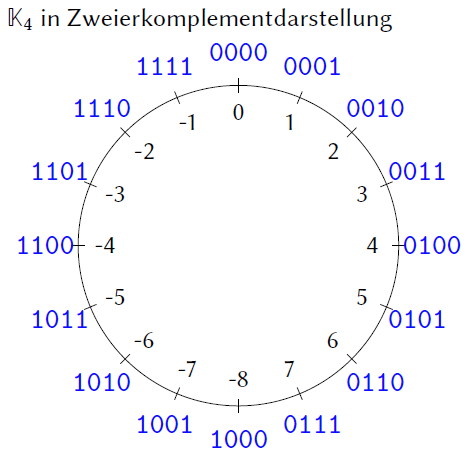
\includegraphics[scale=0.45]{ZK_K4}
	\end{figure}
	
\end{frame}

\begin{frame}{Zweierkomplement}

	Das Zweierkomplement ist eine Möglichkeit, negative Zahlen binär darzustellen. Im Vergleich zu anderen Darstellungsarten ist es besonders vorteilhaft bei arithmetischen Rechnungen mit Hardware \textit{(mehr dazu in Technischer Informatik)}.

	\begin{block}{Definition}
		$$Zkpl_l(x) = \begin{cases} 0 bin_{l-1}(x) & \text{falls } x \geq 0 \\ 1 bin_{l-1}(2^{l-1}+x) & \text{falls } x < 0\end{cases}$$
		
		Äquivalent:
		$$Zkpl_l(x) = \begin{cases} bin_{l}(x) & \text{falls } x \geq 0 \\ bin_{l}(2^{l}+x) & \text{falls } x < 0\end{cases}$$
	\end{block}
\end{frame}

\begin{frame}{ZK-Beispiel}
	\begin{block}{Beispiele}
		\begin{align*}
			&Zkpl_5(0) \only<2->{= 00000} \\
			&Zkpl_5(2) \only<3->{= 00010} \\
			&Zkpl_5(15) \only<4->{= 01111} \\
			&Zkpl_5(-1) \only<5->{= 11111} \\
			&Zkpl_5(-6) \only<6->{= 11010} \\
			&Zkpl_5(-16) \only<7->{= 10000}
		\end{align*}
	\end{block}
\end{frame}

\begin{frame}{ZK: Einfache Berechnung}
	Zum \enquote{intuitiven} Berechnen des Zweierkomplement können wir so vorgehen (für $x < 0$):
	\begin{enumerate}
		\item Binärdarstellung von $\setsize{x}$ berechnen
		\item Mit führenden Nullen auffüllen bis zur Länge $\ell$
		\item Alle binären Ziffern negieren
		\item 1 addieren
	\end{enumerate}

	\begin{Beispiel}
		$$Zkpl_4(-2): 2 \rightarrow 10 \rightarrow 0010 \rightarrow 1101 \rightarrow 1110 $$
	\end{Beispiel}
\end{frame}

\begin{frame}{ZK: Einfache Berechnung}
	Die einzelnen Schritte können wir auch formal angeben:\\
	(Wir operieren jeweils auf Wörtern aus $\{0, 1\}^* = Z_2^*$) \\[0.5em]
	1. Binärdarstellung von $\setsize{x}$ berechnen: $Repr_2(\setsize{\cdot})$ \\
	2. Mit führenden Nullen auffüllen bis zur Länge $\ell$\\ \pause
	\begin{align*}
		Fill_\ell : Z_2^m &\to Z_2^\ell \qquad (m \le \ell) \\ \visible<3-> {
		w &\mapsto \begin{cases}
		0^\ell & w = \varepsilon \\
		Fill_{\ell-1}(w') \cdot \mu & w = w' \cdot \mu, w' \in Z_2^*, \mu \in Z_2
		\end{cases} \\
		&\text{oder deutlich einfacher} \\
		w &\mapsto \begin{cases}
		w & \setsize{w} = \ell \\
		Fill_\ell(0w) & \text{sonst}
		\end{cases} \\
	}
	\end{align*}
	\pause[4] 3. / 4. Analog %TODO
\end{frame}

\begin{frame}{Von einer Zahlendarstellung zur Anderen}
	Eigentlich recht intuitiv:
	$$Trans_{3,5} = Repr_3 \circ Num_5$$
	
	\begin{block}{Aufgabe}
		Berechne folgende Darstellungen:\\
		$Repr_2(42) = \visible<2->{ 101010_2}$ \\
		$Trans_{4,2}(101010) = \visible<3->{ 222_4}$ \\
		$Trans_{8,10}(42) = \visible<4->{ 52_8}$ \\
		$Trans_{16,10}(42) = \visible<5->{ 2A_{16}}$
	\end{block}

	Was ist bei allen Wörtern gleich? \only<6->{Die Bedeutung!} \\
	Was macht die Rechnungen 2 - 4 vergleichsweise einfach? \pause[6] Wir können die Struktur ausnutzen und zeichenweise vorgehen! ($Trans_{8,10}(42) = Trans_{8,2}(101 \cdot 010) = Trans_{8,2}(101) \cdot Trans_{8,2}(010)$)
\end{frame}

\section{Codierungen}

\begin{frame}{Übersetzungen}
	\textbf{Übersetzung:} „Bedeutungserhaltende“ Abbildung \\[0.5em] \pause
	\textbf{Codierung:} Injektive Übersetzung \\ \pause
	\begin{itemize}
		\item Injektiv reicht, weil wir jedem $f(w)$ sein erzeugendes $w$ zuordnen können
		\implitem Definiere Bedeutung von $f(w) := \text{Bedeutung von } w$
	\end{itemize}
	
	\pause
	\begin{itemize}
		\item \textbf{Problem}: \emph{Beliebige} Codierungen zu speichern sehr aufwendig
		\item Wenn $\abs{\text{Definitionsbereich}} = \infty$ \impl sogar unmöglich!
		\implitem Bringen wir etwas Struktur ins Spiel!
	\end{itemize}
\end{frame}

\begin{frame}{Homomorphismen}
	Ein \textbf{Homomorphismus} ist eine \textit{strukturerhaltende} Abbildung \\ \pause
	\begin{threealign}
		\Phi : A &\functionto& B \\
		\text{ mit } \forall x,y \in A: \quad  \Phi(x \sim y) &=& \Phi(x) \bowtie \Phi(y)
	\end{threealign}
	\medskip \\
	Dabei stehen $\sim$ und $\bowtie$ hier für feste beliebige Operationen, wie z.~B. $+, -, \*, /, \oplus, \barwedge, ...$ \\
	(Muss es auf $A$ bzw. $B$ natürlich geben!)
\end{frame}

\begin{frame}{Homomorphismen}
	In GBI: Homomorphismen auf Wörtern mit „$\*$“ als Operation.\\
	\impl $A, B$ Alphabete, dann ist $h: A^* \functionto B^*$ ein Homomorphismus, wenn
	$$ \forall x, y \in A^* : \quad h(x \cdot y) = h(x) \cdot h(y). $$
	
	\pause
	\impl Brauchen nur Funktionswerte für einzelne Zeichen $a \in A$, dann kennen wir schon das ganze $h$! \\
	\impl Brauchen uns nur eine Tabelle für die Zeichen zu merken \\
	\impl $A$ endlich \impl Tabelle endlich \impl gut speicherbar
	
	\pause
	\begin{Beispiel}
		Sei $h$ ein Homomorphismus, für den gilt: $h(\word a) = \word 2, h(\word b) = \word 3$. \\
		Dann gilt $h(\word{aba}) = h(\word a) \cdot h(\word b) \cdot h(\word a) = \word{232}. $ \\[0.5em]
		\pause
		$\fTrans_{16,2}$ ist fast ein Homomorphismus (führende Nullen machen Probleme)\\
		$\fTrans_{3,2}$ ist kein Homomorphismus (siehe dazu ÜB WS15/16)
	\end{Beispiel}
\end{frame}

\begin{frame}{Homomorphismen bauen}
	Haben: Abbildung der einzelnen Zeichen \\
	Wollen: Abbildung ganzer Wörter 
	\begin{Definition}
		Sei $f: A \functionto B^*,$ \pause definiere $f^{**}:A^* \functionto B^*$ als
		\begin{align*}
		f^{**}(\eps) &= \eps  \\
		\forall w\in A^*, x\in A: \quad  f^{**}(w \* x) &= f^{**}(w) \* f(x)       
		\end{align*}
	\end{Definition}

	$f^{**}$ heißt der durch $f$ \textbf{induzierte} Homomorphismus.
\end{frame}

\begin{frame}{$\eps$-Freiheit}
	Klar ist: Für jeden Hom. $h$ ist $h(\eps) = \eps$.
	
	\pause
	\begin{Definition}
		Ein Homomorphismus heißt $\eps$-frei, wenn 	$$ \forall x\in A : h(x) \neq \eps. $$
	\end{Definition}

	
	Was ist das Problem mit Homomorphismen, die nicht $\eps$-frei sind? \\ \pause
	\impl Es geht Information verloren.\\
	
	\begin{Beispiel}
		Sei $h$ ein Hom. mit $h(\word c) = \eps, \; h(\word b) = \word 2$. \\
		Haben unbekanntes $w \in \{\word b, \word c\}^*$ und wissen: $h(w) = \word 2$. \\
		\smallskip
		Wie kommen wir von $h(w)$ wieder zu $w$ zurück? \\ \pause
		\impl Gar nicht! (Wissen nicht, wieviel \word c in $w$ drin sind.)
	\end{Beispiel}
\end{frame}

\begin{frame}{Präfixfreiheit}
	\begin{Definition}
		Ein Homomorphismus heißt \textbf{präfixfrei}, wenn für
		\emph{keine} zwei verschiedenen Symbole $x_1,x_2\in A$ gilt: $h(x_1)$
		ist ein Präfix von $h(x_2)$.
	\end{Definition}

	\bigskip
	Was ist das Problem mit Homomorphismen, die nicht präfixfrei sind? \\ \pause
	\impl Es geht Information verloren.\\
	
	\begin{Beispiel}
		Sei $h$ ein Hom. mit $h(\word a) = \word 2, \; h(\word b) = \word 3, \; h(\word c) = \word{23}$. \\ 
		Haben unbek. $w \in \{\word a, \word b, \word c\}^*$ und wissen: $h(w) = \word{23}$. \\
		\smallskip
		Wie kommen wir von $h(w)$ wieder zu $w$ zurück?\\ \pause
		\impl Gar nicht! $w = \word c$ oder $w = \word{ab}$, wir wissen es nicht!
	\end{Beispiel}
	
\end{frame}

\begin{frame}{Zurück zu Codierungen}
	\begin{block}{Beobachtung}
		Präfixfreie Homomorphismen sind $\eps$-frei.
	\end{block}

	\pause
	\begin{block}{Lemma}
		Präfixfreie Homomorphismen sind Codierungen (also injektiv).
	\end{block}

	\pause
	\begin{block}{Beobachtung}
		Präfixfreie Codes kann man \enquote{einfach} decodieren:
		\[
		u(w) = 
		\begin{cases}
		\eps, & \text{ falls } w=\eps\\
		x\*u(w'), & \text{ falls } w=h(x) \* w' \text{ für ein } x\in A \\
		\bot,  & \text{ sonst }\\
		\end{cases}
		\]
	\end{block}
	($\bot$: „undefiniert“, „bottom“.)
	
\end{frame}

\begin{frame}{Decodierung: Übung}
	\begin{block}{Aufgabe}
	Decodiert das folgende Codewort mit der jeweiligen Codierung:\\
	\word{011000000001}
	\smallskip
	
	(1) $f(\word E) = \word{10} \quad f(\word M) = \word{01} \quad f(\word A) = \word{0001} \quad f(\word T) = \word{0000}$ \\
	\visible<2->{\word{META}} 
	\smallskip
	(2) $f(\word E) = \word 1 \quad f(\word M) = \word 0 \quad f(\word A) = \word{0001} \quad f(\word T) = \word{0000}$ \\
	\visible<3->{Nicht eindeutig möglich, da nicht präfixfrei.}
	\end{block}
\end{frame}

\lastframe{0.5}{0}{xkcd/digital_data.png}{https://www.xkcd.com/1683/}

\section{Huffman-Codierung}

\begin{frame}
	Kann man mit einer Codierung die benötigte Anzahl der Zeichen für ein Wort reduzieren und trotzdem den Sinn erhalten?\\[0.5em]
	\pause
	Natürlich geht das (manchmal), dieses Verfahren ist überall im Einsatz:\\
	Komprimierung!
\end{frame}

\begin{frame}{Huffman-Codierung}
	Eine Huffman-Codierung ist ein präfixfreier (und demnach \enquote{einfach} zu decodierenden) Homomorphismus, bei der die Codierung eines Zeichens umso länger wird, je seltener das Zeichen vorkommt.
	
	Die Huffman-Codierung für ein Wort ist dabei nicht eindeutig, wie wir gleich im Konstruktionsverfahren sehen werden.
	
	\begin{block}{Lemma}
		Unter allen präfixfreien Codes führen Huffman-Codes zu kürzesten Codierungen
		\textbf{des Wortes, für das die Huffman-Codierung konstruiert wurde.}
	\end{block}
\end{frame}

\begin{frame}{Konstruktionsverfahren}
	Formal: In der Vorlesung\\
	Hier: Vorgehensweise (ausreichend!)
	\begin{enumerate}
		\item Für jedes Zeichen die Häufigkeit ermitteln
		\item Alle Zeichen mit ihrer Häufigkeit als Blätter in die unterste Ebene zeichnen
		\item Jeweils die zwei Knoten (nicht unbedingt Blätter!) mit den geringsten Häufigkeiten \enquote{verbinden}(also einen neuen Knoten darüber anlegen, der die Summe der Häufigkeiten erhält)
		\item Fortfahren, bis der ganze Baum aufgebaut ist.
		\item Die linken Äste mit 0 beschriften, die rechten Äste mit 1.
		\item Codierungen der Zeichen ablesen
		\item Ausgangswort codieren (wenn gefordert, vergesst das nicht!)
	\end{enumerate}
\end{frame}

\begin{frame}
	\frametitle{Beispiel}
	Gegeben : $w= abadcadaac $ (10 Zeichen) \\[1em]
	
	\only<1-3|handout:1>{ \visible<3>{
	\begin{minipage}{0.6\linewidth}
		\begin{figure}[b]
			\centering
			\begin{tikzpicture}
			[level 1/.style={sibling distance=40mm},
			level 2/.style={sibling distance=20mm},
			level 3/.style={sibling distance=15mm}]
			\node {$10$}
			child {
				node{$5$}
				child{
					node{$3$}
					child{
						node{$1,b$}
						edge from parent node[left] {\bzero}
					}
					child {
						node{$2,d$}
						edge from parent node[right] {\bone}
					}
					edge from parent node[left] {\bzero};
				}
				child{
					node{$2,c$}
					edge from parent node[right] {\bone}
				}
				edge from parent node[left] {\bzero};
			}
			child{
				node{$5,a$}
				edge from parent node[right] {\bone}
			};
			\end{tikzpicture}
		\end{figure}  
	\end{minipage}
	}}
	\only<4-|handout:2> {
		\begin{minipage}{0.6\linewidth}
			Wie lang wird das neue Wort ?\\ \visible<5->{ 
			$5*1 + 1*3 + 2*2 + 2*3 = 18$ Zeichen\\ 
			Aber wir wollen doch komprimieren? Was haben wir falsch gemacht?\\
			\visible<6->{Nichts. Zur Codierung eines der Zeichen $a, b, c, d$ benötigen wir mindestens 2 Bit (da 4 Möglichkeiten). Für die Zeichen $0, 1$ brauchen wir aber nur ein Bit. \\
			Also haben wir 18 Bit statt 20 Bit und somit komprimiert!
		}}
		\end{minipage}
	}
	\visible<2-> {
		\begin{minipage}{0.2\linewidth}
			\hfill
			\hfill 
			\vspace*{0.1\linewidth}
			\begin{table}[H]
				\begin{tabular}{c|cccc}
					\hline
					x & a & b & c & d  \\ \hline
					$|w|_x$  & 5 & 1 & 2 & 2 \\ \hline
					h(x) & 1 & 000 & 01 & 001 \\ \hline 
				\end{tabular}
			\end{table}
		\end{minipage}
	}
\end{frame}

%TODO: Make solution frame!
\begin{frame}
		Huffman-Codierungen funktionieren immer nur gut für Wörter, die eine gleiche/ähnliche relative Zeichenhäufigkeit haben wie das Wort, für das der Code erstellt wurde.
		
		\begin{Beispiel}
			$w_1 = badcfehg, w_2 = a^1b^2c^4d^8e^{16}f^{32}g^{64}h^{128}$
			Erstellt eine Huffman-Codierung für jedes der beiden Wörter und Codiert jeweils beide Wörter mit der erstellten Codierung.\\
			Wie verhalten sich die Längen der Codewörter?
		\end{Beispiel}
\end{frame}

\begin{frame}
	\begin{block}{Erweiterung}
		Wir können nicht nur einzelne Buchstaben codieren. \\
		Bei $ w = a^{10}b^{10}c^{10} $ lohnt es sich pro Block gleicher Buchstaben eine Codierung zu haben.
	\end{block}
\end{frame}


\subsection{Aufgaben}
\begin{frame}
	\frametitle{Aufgabe (WS 2008) }
	Das Wort $$w = \mathbf{0000\only<3->{\text{ } }0001\only<3->{\text{ } }0011\only<3->{\text{ } }0001\only<3->{\text{ } }0011\only<3->{\text{ } }0000\only<3->{\text{ } }0000\only<3->{\text{ } }1110\only<3->{\text{ } }0001\only<3->{\text{ } }0000}$$ soll komprimiert werden.
	
	\pause
	\begin{itemize}[<+->]
		\item Zerlegen Sie $w$ in Viererblöcke und bestimmen Sie die Häufigkeiten der vorkommenden Blöcke.
		\item Zur Kompression soll ein Huffman-Code verwendet werden. Benutzen Sie die in Teilaufgabe a) bestimmten Häufigkeiten, um den entsprechenden Baum aufzustellen. Beschriften Sie alle Knoten und Kanten.
		\item Geben Sie die Codierung des Wortes $w$ mit Ihrem Code an.
	\end{itemize}
\end{frame}

\begin{frame}
	\frametitle{Lösung}
	$$w = \mathbf{0000000100110001001100000000111000010000}$$
	\textit{Zerlegen Sie $w$ in Viererblöcke und bestimmen Sie die Häufigkeiten der vorkommenden Blöcke.} \\[1em]
	\pause
	$$w = \mathbf{0000 \ 0001 \ 0011 \ 0001 \ 0011 \ 0000 \ 0000 \ 1110 \ 0001 \ 0000}$$ \pause
	\begin{table}[h!]
		\centering
		\begin{tabular}{l|cccc}	
			& 0000 & 0001 & 0011 & 1110 \\ \hline
			Absolute Häufigkeiten: & 4 & 3 & 2 & 1 \\
			Relative Häufigkeiten:  & 0,4 & 0,3 & 0,2 & 0,1\\
		\end{tabular}
	\end{table}
\end{frame}

\begin{frame}
	\frametitle{Lösung}
	\vspace*{1em}
	\begin{minipage}{0.45\linewidth}
		\textit{Zur Kompression soll ein Huffman-Code verwendet werden. Benutzen Sie die in Teilaufgabe a) bestimmten Häufigkeiten, um den entsprechenden Baum aufzustellen. Beschriften Sie alle Knoten und Kanten.}
		\pause 
		\begin{table}[h!]
			\centering
			\begin{tabular}{cccc}	
				0000 & 0001 & 0011 & 1110 \\ \hline
				4 & 3 & 2 & 1 \\	
			\end{tabular}
		\end{table}
	\end{minipage}
	\hfill
	\begin{minipage}{0.5\linewidth}
		\begin{figure}[h!]
			\centering
			\only<3>{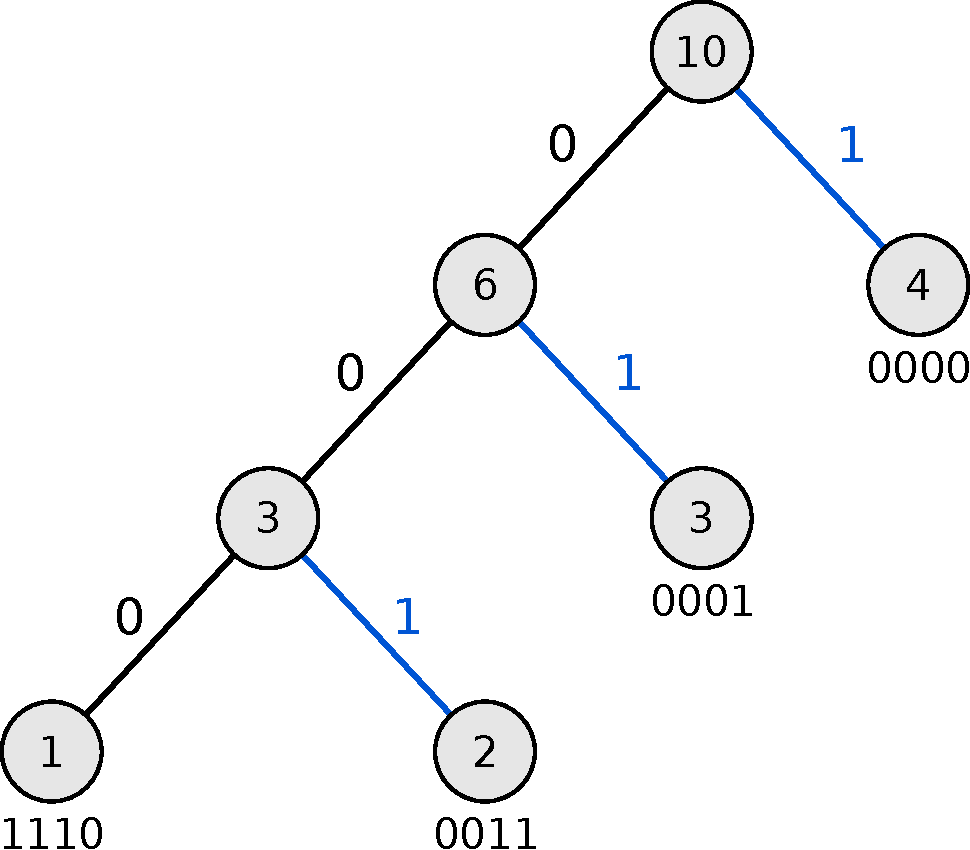
\includegraphics[scale=0.35]{Huffman.pdf}}
		\end{figure}
	\end{minipage}
\end{frame}

\begin{frame}
	\frametitle{Lösung}
	\textit{Geben Sie die Codierung des Wortes $w$ mit Ihrem Code an.} \\[2em] \pause
	$0000000100110001001100000000111000010000$ \\ \hfill $\to 1010010100111000011$
\end{frame}

%\begin{frame}
%	\frametitle{Aufgabe (WS 2010)}
%	Seien $n, k \in \nN_0$ mit $1 \leq k \leq n$. In einem Wort $w \in \{a, b, c\}^\ast$ der Länge $3n$ komme $k$ mal das Zeichen $a$, $n$ mal das Zeichen $b$ und $2n - k$ mal das Zeichen $c$ vor.
%	\begin{itemize}
%		\item Geben Sie den für die Huffman-Codierung benötigten Baum an.
%		\item Geben Sie (in Abhängigkeit von $k$ und $n$) die Länge des zu $w$ gehörenden Huffman-Codes an.
%	\end{itemize}
%\end{frame}
%
%\begin{frame}
%	\frametitle{Lösung}
%	\vspace*{1em}
%	\begin{minipage}{0.45\linewidth}
%		\textit{$\dots$ Länge $3n$ komme $k$ mal das Zeichen $a$, $n$ mal das Zeichen $b$ und $2n - k$ mal das Zeichen $c$ vor. \\[1em] Geben Sie den für die Huffman-Codierung benötigten Baum an.} 
%		\pause
%		\begin{table}[h!]
%			\centering
%			\begin{tabular}{ccc}	
%				$a$ & $b$ & $c$ \\ \hline
%				$k$ & $n$ & $2n-k$ \\	
%			\end{tabular}
%		\end{table}
%		\pause
%		$$k \leq n \leq 2n -k $$ $$ n+k+2n-k = 3n$$
%	\end{minipage}
%	\hfill
%	\begin{minipage}{0.5\linewidth}
%		\begin{figure}[h!]
%			\centering
%			\only<4>{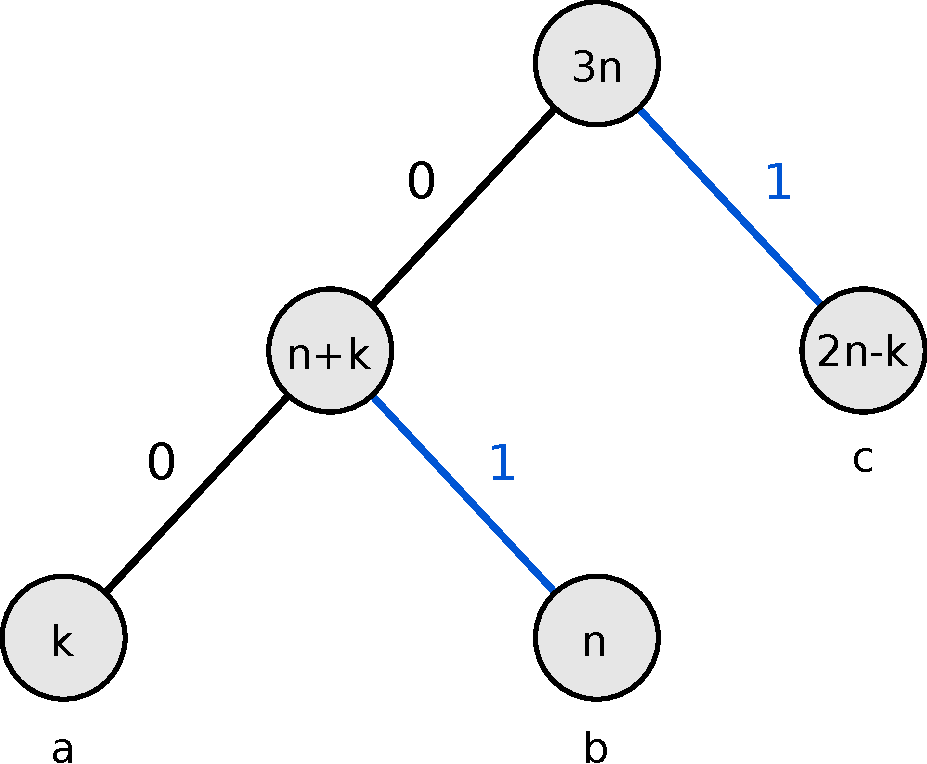
\includegraphics[scale=0.35]{Huffman2.pdf}}
%		\end{figure}
%	\end{minipage}
%\end{frame}
%
%\begin{frame}
%	\frametitle{Lösung}
%	\textit{Geben Sie die Länge des zu $w$ gehörenden Huffman-Codes an.} \\[2em]
%	\pause
%	Jedes $a$ und jedes $b$ wird durch zwei Zeichen codiert, und jedes $c$ wird durch ein Zeichen codiert. Damit erhält man insgesamt $$2k + 2n + 2n - k = 4n + k$$ Zeichen in der Codierung.
%\end{frame}


\begin{frame}{Ausblick}
	Die Huffman-Codierung hat ein Problem: Zum Decodieren muss der Huffman-Baum, der für die Codierung verwendet wurde, bekannt sein. Im wesentlichen gibt es dafür zwei Möglichkeiten:
	\begin{enumerate}
		\item Der Codebaum wird vor dem eigentlichen Codewort angegeben.\\ 
		Problem: Das verlängert das Codewort.
		\item Es wird ein vorher festgelegter Codebaum verwendet.\\
		 Problem: Dieser Codebaum ist nicht an das spezifische Wort angepasst und kann evtl. (bei komplett anderer Zeichenhäufigkeit) zu sehr schlechten Ergebnissen führen.
	\end{enumerate}

	Diese Probleme können durch andere Codierungsverfahren gelöst werden, indem z.B. das Wörterbuch dynamisch während der Decodierung aus dem Codewort aufgebaut wird (z.B. Lempel-Ziv-Welch-Verfahren).
\end{frame}



%\section{Funktionen von Funktionen}

\begin{frame}{Funktionen}
	\begin{Definition}
		Seien A und B Mengen. Dann ist $$B^A := \set{f \Mid f \from A \functionto B }$$ die Menge aller Abbildungen von $A$ nach $B$.
	\end{Definition}

	Abbildungen kann man sich auch als Tabellen vorstellen: \\
	Wir wählen für jedes $a \in A$ ein $b \in B$.
	
	\begin{block}{Beobachtung}
		Für endliche Mengen A und B gilt:
		\delimitershortfall=0pt
		$$\setsize{B^A} = \setsize B^{\setsize A}$$
	\end{block}
\end{frame}

\newcommand{\filter}{filter_{\only<2-3|handout:1>{even}\only<4|handout:2>{odd}\only<5|handout:3>{Uglg}}}

\begin{frame}{Problem: Ziffern filtern}
	Wir wollen aus einer Ziffernfolge (Wort aus $Z^*_{10}$) Ziffern herausfiltern, die eine bestimmte Eigenschaft haben:\\
	\visible<2->{\impl\ }\only<2-3|handout:1>{Gerade}\only<4|handout:2>{Ungerade}\only<5|handout:3>{Löst die Ungleichung $x^2 - 3x < 20$}
	
	\visible<3-> {
		\begin{threealign}
		\filter \from Z^*_{10} &\functionto& Z^*_{10} \\
		\eps &\mapsto& \eps \\
		z \cdot v &\mapsto& \begin{cases}
		z \cdot \filter(v) &\text{falls } \only<2-3|handout:1>{z \in \{\word 2,\word 4,\word 6,\word 8,\word 0\}} \only<4|handout:2>{z \in \{\word 1,\word 3,\word 5,\word 7,\word 9\}} \only<5|handout:3>{z^2 - 3z < 20 }\\
		\filter(v) &\text{sonst}
		\end{cases}\\
		& \multicolumn{2}{l}{\text{wobei } z \in Z_{10} \text{ und } v \in Z_{10}^*.}
		\end{threealign}
	}
\end{frame}

\begin{frame}{Problem: Ziffern filtern}
	\begin{block}{Aufgabe}
		Schreibt die Funktionen zum Filtern aller Ziffern...
		\begin{itemize}
			\item $> 5$
			\item $< 5$
			\item $<2$ oder $>7$
			\item ... die perfekt sind
			\item ... die sich ausmalen lassen
		\end{itemize}
	\end{block}

	\pause
	\impl Blödsinn!\\
	Alle Funktionen unterscheiden sich nur \textbf{an einer Stelle}: \pause \\
	Der \textbf{Bedingung}, die überprüft wird.
\end{frame}

\begin{frame}{Filter}
	Definiere stattdessen eine \textbf{universelle} Filter-Funktion:
	
	\begin{threealign}
		filter_p : Z^*_{10} &\functionto& Z^*_{10} \\
		\eps &\mapsto& \eps \\
		z \cdot v &\mapsto& \begin{cases}
		z \cdot filter_p(v) &\text{falls } p(z) = \W\\
		filter_p(v) &\text{sonst}
		\end{cases}\\
		&\multicolumn{2}{l}{\text{wobei } z \in Z_{10} \text{ und } v \in Z_{10}^*}
	\end{threealign}
	\medskip
	und zwar für alle \quad $p: Z_{10} \functionto \BB$.
\end{frame}

\begin{frame}{Filter}
	\begin{threealign}
		filter_p : Z^*_{10} &\functionto& Z^*_{10} \\
		\eps &\mapsto& \eps \\
		z \cdot v &\mapsto& \begin{cases}
		z \cdot filter_p(v) &\text{falls } p(z) = \W\\
		filter_p(v) &\text{sonst}
		\end{cases}\\
		&\multicolumn{2}{l}{\text{wobei } z \in Z_{10} \text{ und } v \in Z_{10}^*}
	\end{threealign}
	
	Definiere beispielsweise nun:
	$$ even:  Z_{10} \functionto \BB, \; z \mapsto \begin{cases}
	\textbf{w} &\text{falls } z \in \{\word 2,\word  4,\word  6,\word  8,\word  0\}\\
	\textbf{f} &\text{sonst }
	\end{cases}$$
	
	\pause
	Dann ist $filter_{even}(\word{123456}) = \word{246}$.
	
	\smallskip
	\impl Brauchen bloß $p$-Funktionen definieren anstatt jedes Mal ganze Filter-Funktion!
	
\end{frame}

% TOO MUCH FOR THE FIRST TIME, I GUESS...
\mycomment{
	\begin{frame}{Charakteristische Funktion}
		Sei $M$ eine abzählbar unendliche Menge und $L \subseteq M$.
		
		\begin{Definition}
			Die \textbf{Charakteristische Funktion} einer (Teil-)Menge $L$ ist die Funktion 
			\begin{threealign}
			C_L : M &\functionto& \{0, 1\}\\
			x &\mapsto& \begin{cases}
			1 &x \in L \\
			0 &x \notin L
			\end{cases}.
			\end{threealign}
		\end{Definition}
		
		Also ist $C_L \in \{0, 1\}^M$.
		\smallskip
		
		Klar ist außerdem: Es gibt eine Bijektion $C$ zwischen Mengen und Charakteristischen Funktionen: $$C : 2^M \to \{0, 1\}^M, L \mapsto C_L$$
	\end{frame}
	
	\begin{frame}{Charakteristische Funktion}
		Jetzt können wir auf diesen Funktionen äquivalente Operationen wie auf Mengen definieren...
		
		Vereinigung: $V\colon \{0,1\}^M \times \{0,1\}^M\to \{0,1\}^M$\\[1em]
		
		\only<2|handout:1>{
			Beispielbild für $L_1=\{a,c,d\}$ und $L_2=\{b,c\}$
			
			\begin{tabular}{*{4}{>{$}c<{$}}}
				& L_1 & L_2 & L_1\cup L_2 \\
				x & f_1(x) & f_2(x) & V(f_1,f_2) \\
				a & 1 & 0 & 1 \\
				b & 0 & 1 & 1 \\
				c & 1 & 1 & 1 \\
				d & 1 & 0 & 1 \\
				e & 0 & 0 & 0 \\
			\end{tabular}
		}
		
		\only<3-|handout:2> {
			Wie definiert man $V(f_1,f_2)$? Zum Beispiel so:
			\begin{align*}
			V \colon \{0,1\}^M \times  \{0,1\}^M &\to \{0,1\}^M \\
			(f_1,f_2) &\mapsto (x \mapsto \max(f_1(x),f_2(x))) \\
			\end{align*}
		} \only<4|handout:2> {
		Oder so: $V(f_1,f_2) (x) = \max(f_1(x),f_2(x))$
	}
	\end{frame}
}

\newcommand{\yellow}[1]{\fcolorbox{white}{yellow!60}{\ensuremath{#1}}}
\begin{frame}{Funktionen auf LSD: Filter}
	\impl Idee: Mache $p$ zu einem Argument von $filter$!
	\medskip
	\begin{threealign}
		filter \from \yellow{\BB^{Z_{10}} \times } Z^*_{10} &\functionto& Z^*_{10} \\
		(\yellow{p}, \eps) &\mapsto& \eps \\
		(\yellow{p}, z \cdot v) &\mapsto& \begin{cases}
		z \cdot filter(\yellow{p, }v) &\text{falls } p(z) = \W\\
		filter(\yellow{p, }v) &\text{sonst}
		\end{cases}\\
		&\multicolumn{2}{l}{\text{wobei } z \in Z_{10} \text{ und } v \in Z_{10}^*.}
	\end{threealign} \\
	\pause
	
	\impl $filter(even, \word{123456}) = \word{246}$. \\
	\impl $filter(odd, \word{123456}) = \word{135}$.
	\medskip
	
	\impl $filter$ ist jetzt eine Funktion, die \textbf{eine Funktion als Argument} nimmt.
\end{frame}

\newcommand{\fconst}{\text{const}}
\begin{frame}{Funktionen auf LSD: const}
	Schnell: Gebt sieben verschiedene konstante Funktionen an. \\
	\pause
	\impl Zu aufwendig? \visible<6->{\impl Nicht mit \fconst: $\set{\fconst(1),\fconst(2),\fconst(3),...}$}
	\pause
	
	\begin{threealign}
		\fconst \from \R &\functionto& \R^\R \\
		\fconst(a) &:=& \underbrace{\big( x \mapsto a \big)}_{\text{eine Funktion!}}
	\end{threealign} \\
	\pause
	\impl Definiere $f := \fconst(42)$. \quad Dann ist $f(5) = f(1000) = f(-2.3) = 42$. \\
	\smallskip
	\pause
	Oder auch: $\left(\fconst(42)\right)(5) = 42$. \\
	\medskip
	\pause[7]
	
	\impl $\fconst$ ist eine Funktion, die \textbf{eine Funktion als Ergebnis} zurückliefert.
\end{frame}

\begin{frame}
	Wir haben gesehen:
	\begin{itemize}
		\item Eine Abbildung, die eine Funktion auf einen Wert abbildet
		\item Eine Abbildung, die einen Wert auf eine Funktion abbildet
	\end{itemize}
	Gleich werden wir das kombinieren! \\
	\medskip
	(Hinweis: Abbildung $=$ Funktion, gell? \smiley)
\end{frame}

\section{Speicher}

\begin{frame}{Bit vs. Byte}
	\begin{Definition}
		Eine \textbf{Bit} ist ein Zeichen des Alphabets $\{\word 0, \word 1\}$. \\
		Ein Wort aus 8 \emph{Bits} wird \textbf{Byte} genannt. 
	\end{Definition}
	\pause	
	
	\begin{Definition}
		Ein \textbf{Speicher} $$m \from \Adr \functionto \Val$$ bildet Adressen ($\Adr$) auf Werte ($\Val$) ab.\\
		Wir schreiben $\Mem$ für $\Val^\Adr$. \\
		Also: $m \in \Val^{\Adr}$ \quad bzw. \quad $m \in \Mem$.
	\end{Definition}
	\impl Betrachten abstrakte Funktionsweise anstatt konkrete Realisierung 
	%Hier interessiert uns nicht die konkrete Realisierung der Speicherung, sondern nur die abstrakte Funktionsweise.
	\pause
	
	\begin{block}{Hinweis}
		Häufig: Adressen und Werte als Binärzahlen. \\
		%Im Umgang mit Speichern benutzen wir hier nur Zahlen im Binärsystem. \\
		% Zu detailliert:                     und was ist mit negatiuven Zahlen?
		%$\Adr = \set{0, ..., 2^k-1}, \Val = {0,...,2^l-1} \quad \text{für } k,l \in \N_+$.
	\end{block}
\end{frame}

\begin{frame}{Speicher}

	Operationen: \\
	\begin{itemize}
		\item $\memread(m, adr)$, um eine Speicherzelle zu lesen 
		\pause
		\item $\memwrite(m, adr, val)$, um in eine Speicherzelle zu „schreiben“.  
	\end{itemize}
	
	\pause
	\begin{threealign}
		\memread \from \Val^{\Adr} \times \Adr &\functionto& \Val \\
		(m,a) &\mapsto& m(a)  \medskip  
		\visible<4->{ \\
			\memwrite \from \Val^{\Adr} \times \Adr \times \Val &\functionto& \Val^{\Adr} \\
			(m,a',v') &\mapsto& m' , \quad \text{wobei} 
		} 
		\visible<5->{ \\ 
				m'(a) &=&
				\begin{cases}
				v' & \text{ falls } a=a' \\
				m(a) & \text{ falls } a\not=a' \\
				\end{cases}	
		}
	\end{threealign}	
	\pause[6]
	$\memwrite$ gibt die neue Speichertabelle $m'$ zurück!
\end{frame}

\begin{frame}{Speicher}
	\begin{block}{Beispiel}
		
	$\memread(m, \word{01}) = \only<2->{\word{00000111}}$\\
	\visible<2-|handout:2>{$m' := \memwrite(m, \word{01}, \word{11111100})$\\}
	\visible<3-|handout:2>{$\memread\big(\underbrace{\memwrite(m, \word{01}, \word{11111100})}_{m'}, \word{01}\big) = \word{11111100}$\\}
	\bigskip
	
	\begin{table}
		\begin{tabular}{r}
			\\ \\ \\ \\  \\
			\visible<4-|handout:2>{Realworld-Analogie: }
		\end{tabular}
		\begin{tabular}{|c|c|}
			\hline
			\multicolumn{2}{|c|}{Speicher $m$} \\
			\hline
			\word{00} & \word{00101000} \\
			\word{01} & \word{00000111} \\
			\word{10} & \word{10010110} \\
			\word{11} & \word{00100101} \\ 
			\hline 
			\multicolumn{2}{c}{\visible<4-|handout:2>{Zustand bei $t=0$}}
		\end{tabular} 
		\visible<2-|handout:2>{
			\begin{tabular}{|c|c|}
				\hline
				\multicolumn{2}{|c|}{Speicher $m'$} \\
				\hline
				\word{00} & \word{00101000} \\
				\underline{\word{01}} & \underline{\word{11111100}} \\
				\word{10} & \word{10010110} \\
				\word{11} & \word{00100101} \\
				\hline
				\multicolumn{2}{c}{\visible<4-|handout:2>{Zustand bei $t=1$}}
			\end{tabular} 
		}
	\end{table}

	\end{block}
\end{frame}

\only<handout:0>{\begin{frame}{Aufgaben}
	
\end{frame}}

\begin{frame}	
	\begin{block}{Was ihr nun wissen solltet}
		\begin{itemize}
			\item Wie man das Zweierkomplement bildet
			\item Übersetzungen und Codierungen
			\item Huffman-Codierung
		\end{itemize}
	\end{block}
	
	\begin{block}{Was nächstes Mal kommt}
		\begin{itemize}
			\item Speicher - Damit wir nicht alles gleich wieder vergessen
			\item MIMA - Den Bits beim Arbeiten zuschauen
		\end{itemize}
	\end{block}
\end{frame}

\lastframe{0.75}{0}{xkcd/tar.png}{https://www.xkcd.com/1168/}
\slideThanks

\end{document}